\documentclass[12pt, a4paper]{article}
\usepackage[utf8]{inputenc}
\usepackage[english]{babel}
\usepackage{amsmath}
\usepackage{amsfonts}
\usepackage{amssymb}
\usepackage{csquotes}
\usepackage{mathtools}
\usepackage{graphicx}
\usepackage{geometry}
\usepackage{setspace}
\usepackage{longtable}
\usepackage{float}
\usepackage{comment}
\usepackage{listings}
\usepackage{fancyhdr}
\usepackage{blindtext}
\usepackage[colorlinks=true, allcolors=blue]{hyperref}

\usepackage[style=authoryear]{biblatex}
\addbibresource{Bibliography.bib}

\geometry{top = 2.5cm, bottom = 2.5cm, left= 3cm, right= 3cm}

\fancypagestyle{mystyle}
{
    \rhead{Experiment 16}
    \lfoot{Lee Farrugia}
    \cfoot{}
    \rfoot{Page \thepage}
    \renewcommand{\headrulewidth}{0pt}
    \renewcommand{\footrulewidth}{0.5pt}
}

\fancypagestyle{titlepagestyle}
{
    \fancyhf{}
    \lfoot{Lee Farrugia}
    \cfoot{}
    \rfoot{Page \thepage}
    \renewcommand{\headrulewidth}{0pt}
    \renewcommand{\footrulewidth}{0.5pt}
}

\title{The specific charge of electrons}
\author{Lee Farrugia \\ Experiment 16 \\ Group 1A}

\date{25$^{\text{th}}$ February 2022}

\begin{document}

\maketitle
\thispagestyle{titlepagestyle}
\pagestyle{mystyle}

\section*{Aim}
This experiment was done in order to determine the specific charge of electrons by magnetic deflection.

\section*{Diagram}
\begin{figure}[H]
    \centering
    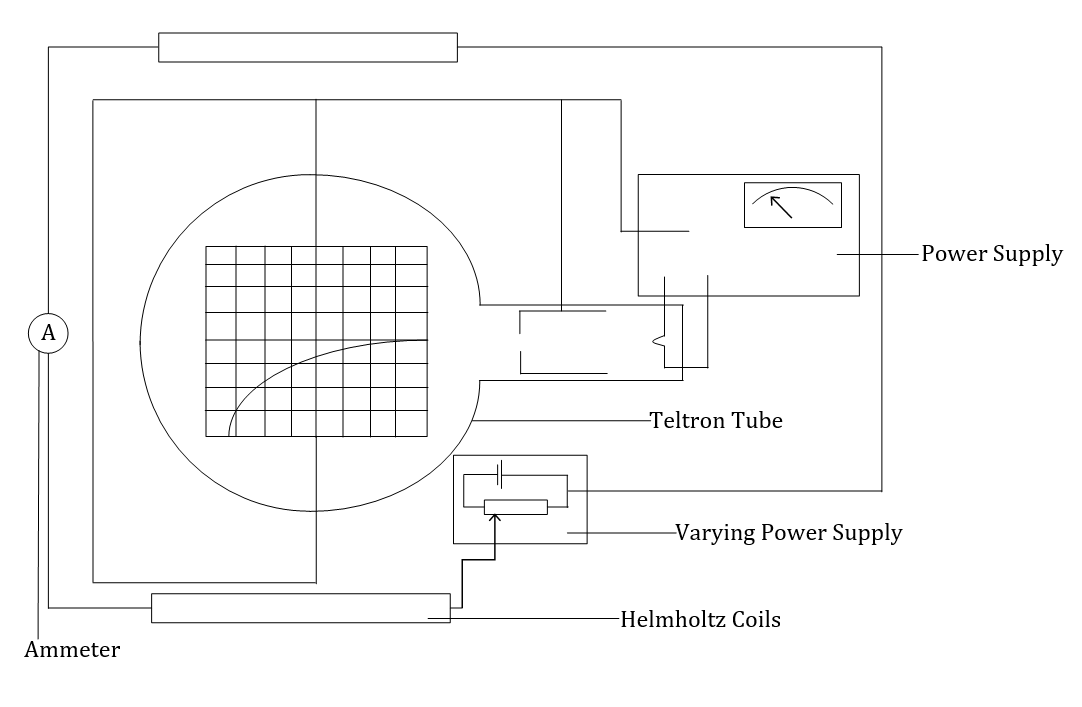
\includegraphics[width=\textwidth]{Experiment 16 diagram.png}
    \caption{Apparatus Setup}
    \label{fig:Set up}
\end{figure}

\section*{List of Apparatus}
Teltron Tube(containing of an electron gun with cathode  and anode , fluorescent graduated scale and plates), Helmholtz coil, extra high tension electrical supply, low voltage supply, variable d.c. voltage supply, ammeter

\section*{Language and Packages}
Python 3.9.7, Numpy, Matplotlib.pyplot, Pandas, Sympy, Math

\section*{Procedure}
\begin{enumerate}
    \item The heater supply of 6.3 V was switched on, after which the voltage supply of the anode was set to 1.5 kV. A horizontal luminous beam was seen on the graduated screen along its \textit{x}-axis.
    \item The circuit supplying the current for the Helmholtz coils was switched on and the beam was observed to be deflected along a circular arc.
    \item The current passing through the coils was adjusted such that the arc was passing through a point where the vertical and horizontal lines intersect. The coordinates of the points were recorded in table below along with the current of the Helmholtz coils $I$ up to 0.75 A.
    \item The experiment was repeated until four sets of data were obtained, alternating in increasing and decreasing values of $I$.
    \item A linear graph was plotted using the data in order to obtain the specific charge of electrons.
\end{enumerate}

\section*{Precautions}
\begin{itemize}
    \item[-] A separate galvanometer was used in order to read the current flowing through the coils in order to reducing fluctuations.
    \item[-] Care was taken to  not move the coils while the apparatus was switched on.
    \item[-] Care was taken to not exceed the maximum current value for the coils.
    \item[-] The current readings were taken in an alternating manner.
    \item[-] Readings from the ammeter were taken at eye level.
\end{itemize}

\section*{Sources of Error}
\begin{itemize}
    \item[-] Parallax error when reading the coordinates on the graduated scale.
    \item[-] Beam of light was not narrow at the extremities.
    \item[-] The beam of light as not directly on the 0 lines of the $x$-axis and $y$-axis.
    \item[-] Ammeter does not have zero resistance.
    \item[-] Resistance of the wires were ignored. 
\end{itemize}

\section*{Data and Graphs}
\begin{longtable}{|c|c|c|c|c|c|}
\hline $x$/m & $y$/m & $CH_{\text{1}}$/A & $CH_{\text{2}}$/A & $CH_{\text{3}}$/A & $CH_{\text{4}}$/A \\
\hline \textpm 0.001 & \textpm 0.001 & \textpm 0.01 & \textpm 0.01 & \textpm 0.01 & \textpm 0.01\\ \hline
\endfirsthead

\hline $x$/m & $y$/m & $CH_{\text{1}}$/A & $CH_{\text{2}}$/A & $CH_{\text{3}}$/A & $CH_{\text{4}}$/A \\
\hline \textpm 0.001 & \textpm 0.001 & \textpm 0.01 & \textpm 0.01 & \textpm 0.01 & \textpm 0.01\\ \hline
\endhead

0.038 & 0.008 & 0.38 & 0.38 & 0.38 & 0.39 \\ \hline
0.045 & 0.008 & 0.25 & 0.26 & 0.25 & 0.26 \\ \hline
0.055 & 0.008 & 0.18 & 0.18 & 0.18 & 0.18 \\ \hline
0.065 & 0.008 & 0.12 & 0.14 & 0.13 & 0.13 \\ \hline
0.075 & 0.008 & 0.10 & 0.10 & 0.10 & 0.10 \\ \hline
0.085 & 0.008 & 0.08 & 0.08 & 0.08 & 0.08 \\ \hline
0.095 & 0.008 & 0.06 & 0.06 & 0.06 & 0.06 \\ \hline

\caption{Coordinates and Corresponding Currents}
\label{tab:Table 1}\\
\end{longtable}

\begin{figure}
    \centering
    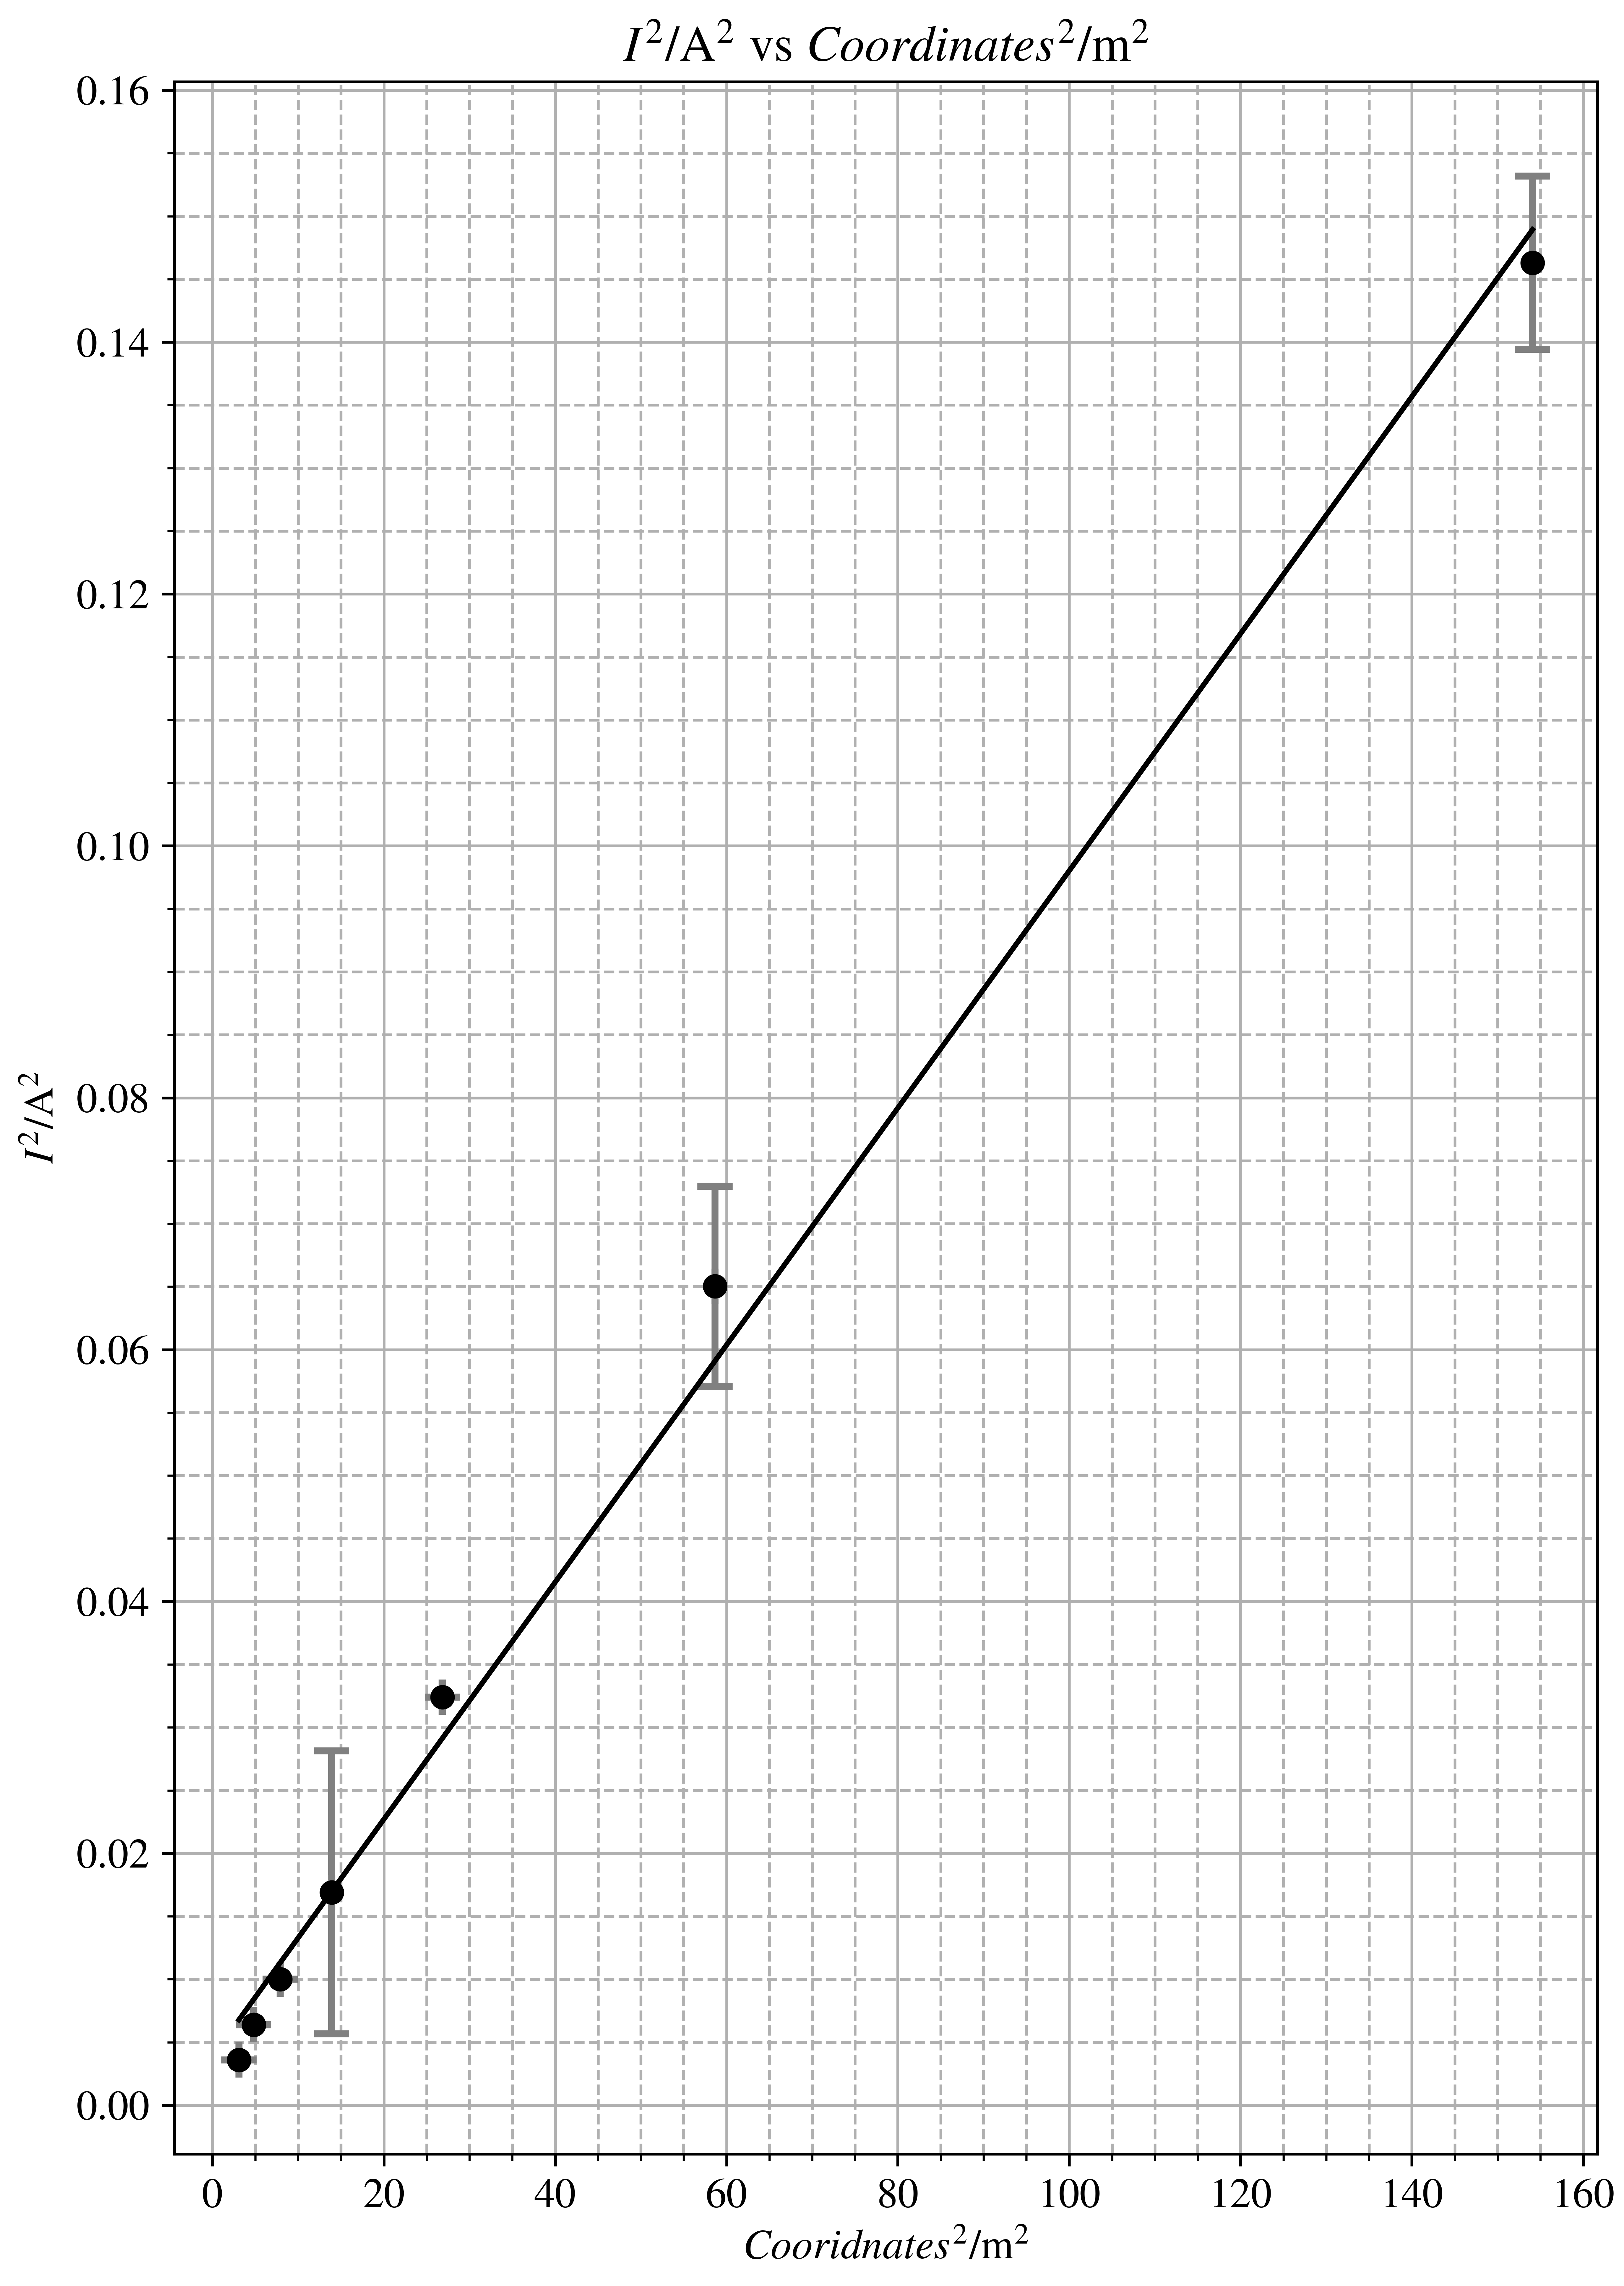
\includegraphics[width=\textwidth]{I2vsCo-or2.png}
    \caption{Graph of Current vs the coordinates}
    \label{fig:I2vsCoor}
\end{figure}

\section*{Calculations}
The data collected during the experiment was imported into the program from the excel sheet, by using the following line of code:
\begin{lstlisting}
    data = pd.read_excel(`Experiment 16.xlsx').
\end{lstlisting}
The coordinates of where the beam was passing through intersecting points of $x$ and $y$ axes where defined as array and changed into meters by the following lines of code:
\begin{lstlisting}
    x = np.asarray(data[`x'])/100
    y = np.asarray(data[`y'])/100,
\end{lstlisting}
while the average of the corresponding point was found with the following line of code:
\begin{lstlisting}
    I = np.asarray(0.25 * (data[`CH1'] + data[`CH2'] + 
                   data[`CH3'] + data[`CH4'])).
\end{lstlisting}
The constants that were given were defined by using the following lines of code:
\begin{lstlisting}
    V = 1500
    r = 0.065
    N = 320
    u = 1.257e-6
    ae = 1.76e11.
\end{lstlisting}
The equation given in order to find the specific charge of electrons is:
\begin{equation*}
    \frac{e}{m_{\text{e}}} = \frac{2\text{V}\text{r}_{\text{H}}^2}{0.72^2\mu_0^2\text{N}^2}\left[\frac{1}{I}\left(\frac{2y}{x^2 + y^2}\right)\right]^2\,,
\end{equation*}
where $\frac{e}{m_e}$ is the specific charge of electrons, V is the anode voltage, $\text{r}_H^2$ is the radius of the Helmholtz coils, $\mu_0^2$ is permeability of vacuum, $\text{N}^2$ is the number of turns in the coils, $I$ is the current passing through the coils and x and y are the coordinates on the scale. The equation was rearranged in order to make it fit to the straight line equation $y=\text{m}x+\text{c}$, and became:
\begin{equation*}
    I^2 = \frac{e}{\text{c}m_e}\left(\frac{2y}{x^2 + y^2}\right)^2 \,,
\end{equation*}
where c is the constant:
\begin{equation*}
    \frac{2\text{V}\text{r}_{\text{H}}^2}{0.72^2\mu_0^2\text{N}^2}\,.
\end{equation*}
Thus $I^2$ corresponds to y, $\frac{e}{\text{c}m_e}$ corresponds to m, and $\left(\frac{2y}{x^2 + y^2}\right)^2$. The corresponding y and x where given the variable names of Y and X respectively in the program. These were then plotted against each other in order to obtain a straight line fitted to the data. This was done by first finding the equation of the line of best fit to the data and the inputting the data points in order to obtain the line of best fit. This was done using the following lines of code:
\begin{lstlisting}
    coeffs, cov = np.polyfit(X, Y, 1, cov=True)
    poly_function = np.poly1d(coeffs)
    trendline = poly_function(X).
\end{lstlisting}
As the gradient contains the specific charge of electrons is was defined by calling the relevant position in the coeffs array by:
\begin{lstlisting}
    m = coeffs[0],
\end{lstlisting}
and its error was found by square rooting the relevant position of the co-variance matrix by:
\begin{lstlisting}
    dm = np.sqrt(cov[0][0]).
\end{lstlisting}
from this the gradient was found to be $0.0009 \pm 2.77\times10^{-5}\mathrm{ A}^2/\mathrm{m}^2$. Therefore in order to obtain the specific charge of electrons the gradient was then multiplied by the constant defined previously called c which resulted in the value of specific charge of electrons to be $1.61\times10^{11} \pm 4.73\times10^9$ CKg$^{-1}$. The error for the specific charge of electrons was obtained by doing the partial derivative of the gradient as follows:
\begin{equation*}
    \frac{\partial\frac{e}{m_e}}{\partial m}=\left|{-\frac{1}{m^2}}\right|\Delta m\,,
\end{equation*}
which was done through the program using the following lines of code:
\begin{lstlisting}
    def merr(d, e, dm):
        a = Symbol(`a')
        b = Symbol(`b')
        equation = a/b
        diff_b = Derivative(equation, b)
        db = diff_b.doit()
        de = db.subs({a : c, b : m}).evalf()
        return de*dm
    de = abs(merr(c, m, dm)).
\end{lstlisting}
The error bars for each point of the data was dived in to two systems. The error bars for the X coordinates was 0.01 m as there was no standard deviation for the points used as coordinates, therefore the the minimum readability of the scale was used. However, in order to obtain the error bars for the current, the standard deviation was found by using the following lines of code:
\begin{lstlisting}
    dI = 3.18 * np.std([data[`CH1'], data[`CH2'], 
                        data[`CH3'], data[`CH4']],
                        axis=0)/np.sqrt(4),
\end{lstlisting}
it was noted that the standard deviation was done on the 0 axis as the data was inputted in a row manner rather than a column manner. The precision and accuracy are given by the following equations:
\begin{align*}
    \text{Precision}&=\frac{\text{Combined Error}}{\text{Experimental Value}} \times 100\% \\
    \smallskip
    \text{Accuracy} &= \frac{\text{Experimental Value}}{\text{Actual Value}} \times 100\% \,,
\end{align*}
these were applied through the program with following lines of code:
\begin{lstlisting}
    precision = (de/e) * 100
    accuracy = (e/ae) * 100.
\end{lstlisting}
It was found that the value of the specific electron charge had a precision of 2.95\% and an accuracy of 91.20\%.

\section*{Discussion}
The specific charge of electrons was found to be $1.61\times10^{11}\pm4.73\times10^9$ CKg$^{-1}$ while the actual value is $1.76\times10^{11}$ CKg$^{-1}$. This resulted in a precision value of 2.95\% and an accuracy value of 91.20\%. The values indicate that the result obtained was very accurate when compared to the actual value, while also the 2.95\% precision value indicated that the data collected was done in a very precise manner. This is due to the precautions taken during the experiment.This is also reflected in fact that the error bars in the graph are quite small.
\smallskip

\noindent
The Teltron Tube works by having a hot cathode that passes a 6.3V through a tungsten wire. This produces the electron beam which as it is passing over the mica screen, gives off light on its pathway \parencite{Strawson_2009}.In order to move electrons from the tungsten into the vacuum of the tube energy is required and supplied by the power supply. This is due to the Boltzmann equation:
\begin{equation*}
    N = N_0 \text{e}^{-\frac{E}{kt}}\,,
\end{equation*}
where $N$ is the number of electrons in the vacuum, $N_0$ is the number of electrons in the metal, $E$ is the energy required to move the electrons from the metal to the vacuum, $k$ is Boltzmann's constant and $t$ is time \parencite{Strawson_2009}.
\smallskip

\noindent
The Helmholtz coils work by creating a magnetic field between the two coils. In order for the optimal magnetic field to be formed, the distance between the two coils should be the same length as the radius of the coils. The coils generate a uniform field in in the center, which nullifies any effect the earth magnetic field may have on the electron beam being projected from the tube \parencite{doi:10.1063/1.3474227}. 

\section*{References:}
\printbibliography[heading=none]

\section*{Appendix}
\lstset{language=Python,
    showstringspaces=false,
    showtabs=false}
\begin{lstlisting}
import numpy as np
import pandas as pd
import matplotlib.pyplot as plt
from sympy import *
from math import sqrt

# importing data and defining constants
data = pd.read_excel(`Experiment 16.xlsx')
x = np.asarray(data[`x'])/100
y = np.asarray(data[`y'])/100
V = 1500
I = np.asarray(0.25 * (data[`CH1'] + data[`CH2'] + 
               data[`CH3'] + data[`CH4']))
r = 0.065
N = 320
u = 1.257e-6
ae = 1.76e11

# defining the constant
c = ((2*V*r**2)/(0.72**2 * u**2 * N**2))
# defining the co-oridnate values
X = np.array(((2*y)/(x**2 + y**2))**2)
Y = np.array(I**2)
# defining the error for I
dI = 3.18 * np.std([data[`CH1'], data[`CH2'], 
                    data[`CH3'], data[`CH4']],
                    axis=0)/np.sqrt(4)
# as std=0 minimum readability is used
dX = 0.01

# finding the equation of the line of best fit
coeffs, cov = np.polyfit(X, Y, 1, cov=True)
poly_function = np.poly1d(coeffs)
# defining the line of best fit
trendline = poly_function(X)
# definfing the value of the gradient
m = coeffs[0]
# finding the error of the gradient
dm = np.sqrt(cov[0][0])

# calculating the specific charge of an electron
e = c/(m)

# doing the partial derivative
def merr(d, e, dm):
    a = Symbol(`a')
    b = Symbol(`b')
    equation = a/b
    diff_b = Derivative(equation, b)
    db = diff_b.doit()
    de = db.subs({a : c, b : m}).evalf()
    return de*dm
de = abs(merr(c, m, dm))
print(f`The specific charge of electrons is {e:.2e}, 
        with an error of {de:.2e}')
# finding the precision and accuracy of the values of 
    the value obtained
precision = (de/e) * 100
accuracy = (e/ae) * 100
print(f`With a precision of {precision:.2f}% 
        and an accuracy of {accuracy:.2f}%')

# defining the fonts and sizes to be used
plt.rcParams[`font.family'] = `STIXGeneral'
plt.rcParams[`mathtext.fontset'] = `stix'
plt.rcParams[`font.size'] = 12
plt.rcParams[`font.weight'] = `normal'

# defining the size of the figure
f = plt.figure(figsize=(7.3, 10.7))

# defining the plot and showing it
plt.errorbar(X, Y, xerr=dX, yerr=dI, fmt=`o', color=`k', 
             elinewidth=2, capthick=2, capsize=5,
             ecolor=`grey', label=`Data Points')
plt.plot(X, trendline, color=`k', label=`Fit')
plt.minorticks_on()
plt.grid(b=True, which=`major', linestyle=`-')
plt.grid(b=True, which=`minor', linestyle=`--')
plt.xlabel(r`$Co$-$oridnates^2$/m$^2$')
plt.ylabel(r`$I^2$/A$^2$')
plt.title(r`$I^2$/A$^2$ vs $Co$-$ordinates^2$/m$^2$')
plt.savefig(`I2vsCo-or2.png', dpi=800)
plt.legend()
plt.show()
\end{lstlisting}

\end{document}
